% Chapter Template
\chapter{Introduction}

\label{Introduction}

Neural networks designed for a classification task typically map inputs coming from a very high-dimensional space to a rather low-dimensional space - the space of possible classes.
$$
x \in \R^n,\ y \in \R^m ,\ n \gg m
$$
$$\phi (x) = y
$$
Given the nature of such a task, this forward process typically incurs in a huge loss of information. When $n > m$ and the data is not contained in some lower-dimensional submanifold, then the restriction of the map $\phi$ to the data manifold can not be bijective and therefore not invertible. 
Thus, given only the output, it is generally not possible to recover the input.
Typically, this transformation of the input to more abstract, meaningful features, along with the resulting compression is desired. Yet, the inverse problem of accurately modeling the posterior distribution $p(x|\;y)$ or an approximation thereof is an active area of research with many applications.
Such advantages of invertibility can be more efficient training, knowledge distillation in teacher-student networks, but also most notably, interpretability of a neural network's decision process - a big concern in security-related fields such as medical sciences, autonomous vehicles and face-recognition. 

Some recent work in this area are \textit{Invertible Neural Networks} \citep{ardizzone2018analyzing} , \textit{Glow: Generative Flow with Invertible 1x1 Convolutions} \citep{kingma2018glow} and \textit{Invertible Residual Networks} \citep{behrmann2018invertible}. The methods used vary from noise-optimization, direct parametrization to solving fixed-point iterations.

For the sake of interpretability, it is often enough to be able to sample from the posterior distribution.
The method that will be further examined in this work is an iterative refinement-process that optimizes random noise or an existing image to meet some criterion. This method was made popular by the computer vision program \textit{DeepDream} \citep{DeepDream} and later further improved on by \textit{DeepInversion} \citep{DeepInversion}.

\chapter{Feature Regularization} % Main chapter title

\label{Chapter2} % Change X to a consecutive number; for referencing this chapter elsewhere, use \ref{ChapterX}

%----------------------------------------------------------------------------------------
%	SECTION 1
%----------------------------------------------------------------------------------------

The basic idea used for dataset-reconstruction will be illustrated using a neural network trained for a simple classification task on a two-dimensional toy dataset. The same principle can be applied to image-classification networks, although intuition does not always hold in the very high-dimensional setting.

\begin{figure}
\centering
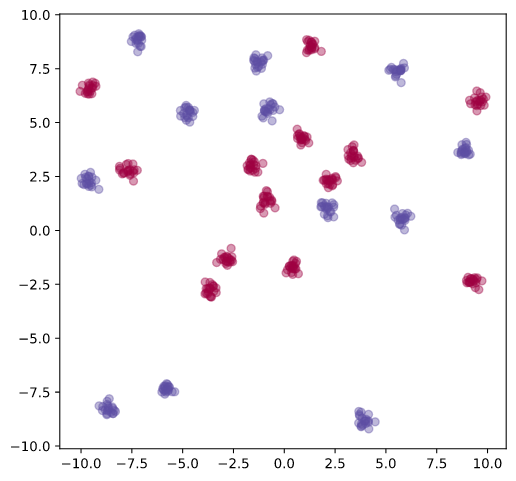
\includegraphics[width=0.5\textwidth]{Figures/toy_dataset.png}
\decoRule
\caption{toy dataset}
\label{fig:toy_dataset}
\end{figure}

%Given a dataset consisting of multiple classes, each with distinct features (as seen in \ref{fig:toy_dataset}), a neural network designed for the task of classification can generally (given that the  network is expressive enough) be trained to attain a high accuracy for this task.

\begin{figure}
\centering
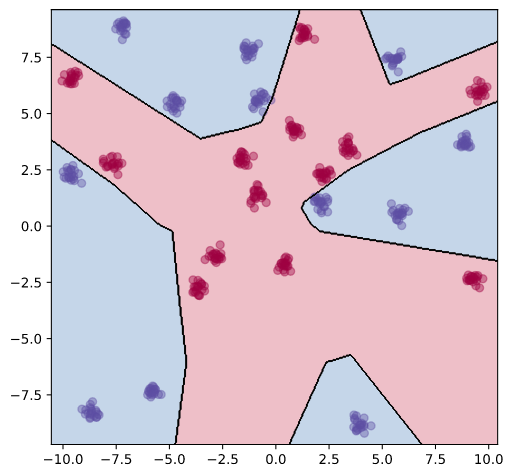
\includegraphics[width=0.5\textwidth]{Figures/toy_dataset_contour.png}
\decoRule
\caption{prediction by the neural network}
\label{fig:toy_dataset_contour}
\end{figure}

In the case of a two-dimensional dataset (as seen in \ref{fig:toy_dataset}), the predicted outcome of the neural network for any given point and the decision boundary can easily be visualized, as shown in \ref{fig:toy_dataset_contour}.
Here, a fully-connected neural network with two hidden layers of dimensions 8 and 6 was trained using the cross-entropy loss function to achieve a 100\% correct classification rate.

A method for reconstructing a data-point of a certain target-class $\hat y$, given only the neural network, is to start with a randomly initialized point in the input-space and then incrementally tweak it to maximize the neural network's response for the given class $\hat y$. In the same fashion as updating the weights of the network by gradient descent to minimize the error, the point can be updated instead to reach a lower classification-error.
This corresponds to minimizing the loss $\mathcal L$, given $\hat y$  with respect to the input $x$.
$$\min_x \mathcal L (x,\hat y)
$$

\begin{figure}
\centering
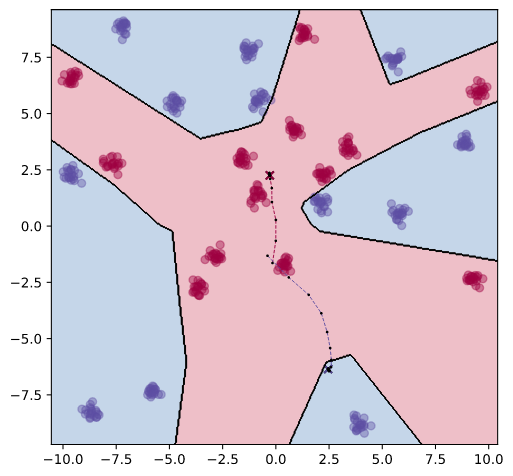
\includegraphics[width=0.5\textwidth]{Figures/toy_dataset_invert.png}
\decoRule
\caption{dataset-reconstruction}
\label{fig:toy_dataset_invert}
\end{figure}

The path such a data point might undertake in the optimization-process is shown in \ref{fig:toy_dataset_invert}.
In this setting, in order to gain further insight, the loss that is being optimized for can be plotted for each class individually. The resulting scalar-field is shown in  \ref{fig:toy_dataset_loss_landscape} and will be referred to as the \textit{loss-landscape}.

\begin{figure}
\centering
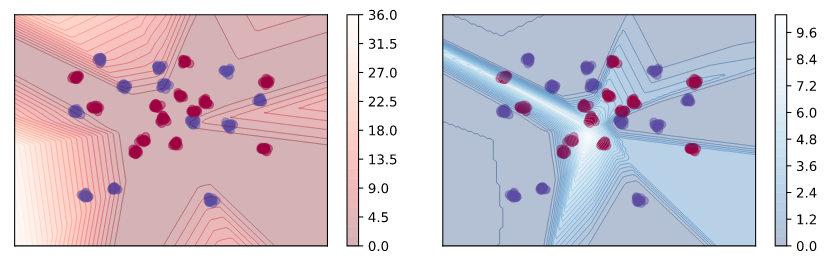
\includegraphics[width=\textwidth]{Figures/toy_dataset_loss_landscape.png}
\decoRule
\caption{loss-landscape}
\label{fig:toy_dataset_loss_landscape}
\end{figure}

Through this visualization it becomes clear that the points in \ref{fig:toy_dataset_invert} are moving toward local minima in the loss-landscape.
Some issues that are already foreseeable with this method is that the resulting end-points can (and in the most cases will) be chaotic with respect to the initialization. Points that are initially "close" can result in very different outcomes. It is also not immediately clear how many iteration-steps to perform or what criterion for stopping to meet when reconstruction is performed.
Another problem could be that points might "trail off" from the dataset-cluster or that points starting further away might keep their distance during the optimization-process. These points might be given a high score for belonging to the target-class by the network, yet they might not share the same statistics as "natural" data-points. This is seen in \ref{fig:toy_dataset_invert} as the reconstructed points don't end up near the clusters.

A way to combat this is to enforce similar statistics as those of the original dataset by including a regularization-term $\mathcal R$. In order to perform this, statistics, such as the mean and variance need to be tracked as additional parameters of the network (this can be done during training-time or once after training).
The statistics can be recorded for the whole dataset or for each class individually.
\cite{DeepInversion} have shown that using the statistics (mean and variance) stored in the batch-norm-layers of residual-networks can already greatly improve the reconstruction quality of images.
The advantage here is that these statistics are already included in a highly-utilized framework and are readily available without further labor. 

In the simple case of the toy-dataset, $\mathcal R$ could be formulated as
$$\mathcal R(x,\hat y) := \|x-\bar x_{\hat y}\|_2^2
\comma$$
where $\bar x_{\hat y}$ is the mean of class $\hat y$. Here, the variance has been omitted for simplicity.

\begin{figure}
\centering
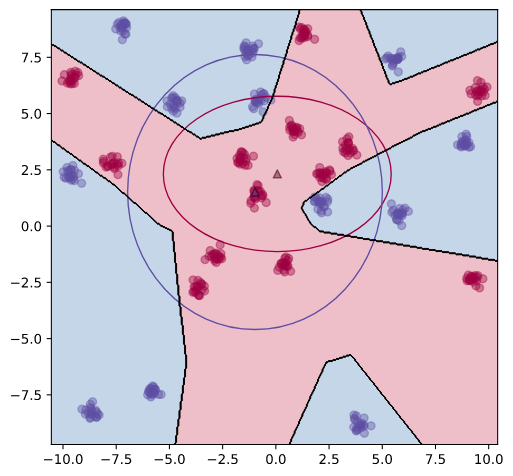
\includegraphics[width=0.5\textwidth]{Figures/toy_dataset_stats.png}
\decoRule
\caption{class-specific mean and variance}
\label{fig:toy_dataset_stats}
\end{figure}

Again, the effect of the additional regularization-term for each class can be made visible by plotting the resulting loss-landscape of $\mathcal R$, as seen in \ref{fig:toy_dataset_loss_stats}, which should reflect the class-dependent statistics.
\XXX{You used variance statistics for plotting}

\begin{figure}
\centering
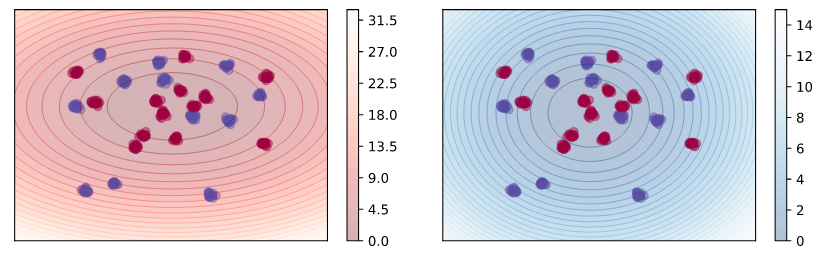
\includegraphics[width=\textwidth]{Figures/toy_dataset_loss_stats.png}
\decoRule
\caption{loss-landscape of the class-dependent regularization-term}
\label{fig:toy_dataset_loss_stats}
\end{figure}

The regularization may be incorporated in the loss by simply adding the new term (multiplied by a factor) to the original loss-formulation.
$$\min_x \mathcal L (x,\hat y) + \mathcal R(x,\hat y)
$$
The loss-landscape of the combination is shown in \ref{fig:toy_dataset_loss_combined}.

\begin{figure}
\centering
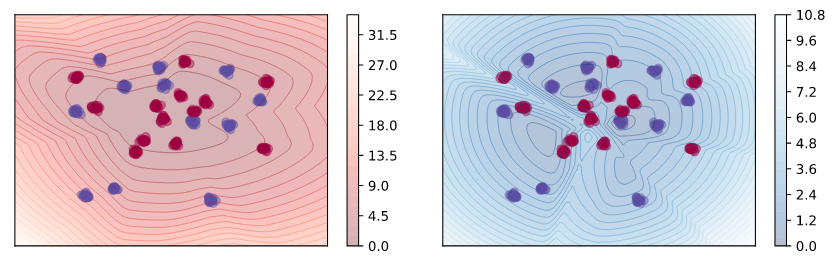
\includegraphics[width=\textwidth]{Figures/toy_dataset_loss_combined.png}
\decoRule
\caption{combined loss-landscape}
\label{fig:toy_dataset_loss_combined}
\end{figure}

So far, only the class-dependent statistics of the dataset have been taken into account. These statistics can be viewed as the statistics of the input to the first hidden layer of the neural network. In the same manner, the statistics of the input to subsequent layers of the network can be tracked and included in the regularization-term with an individual weighting.
$$\mathcal R(x,\hat y) := 
\lambda_0 \|x-\bar x_{\hat y}\|^2 
+ \lambda_1 \|\phi^{(1)} (x)-\bar x_{\hat y}^{(1)}\|^2
+ \lambda_2 \|\phi^{(2)} (x)-\bar x_{\hat y}^{(2)}\|^2
+ \ldots
\comma$$

where $\phi^{(i)}$ is the network's output of the $i$-th hidden layer and $\bar x_{\hat y}^{(i)}$ is the mean of $\phi^{(i)}$ over the data of the target-class $\hat y$.

$$\mathcal R(x,\hat y) := 
\sum_{i=0}^L \lambda_i \|\phi^{(i)} (x)-\bar x_{\hat y}^{(i)}\|^2
\comma$$
for a network with $L$ hidden layers, and where $\phi^{(0)}(x) := x$ and $\bar x_{\hat y}^{(0)} := \bar x_{\hat y}$.
$\lambda_i$ are seen as additional hyper-parameters.

%%-----------------------------------
%%	SUBSECTION 1
%%-----------------------------------
%\subsection{Subsection 1}
%
%
%
%%-----------------------------------
%%	SUBSECTION 2
%%-----------------------------------
%
%\subsection{Subsection 2}
%
%%----------------------------------------------------------------------------------------
%%	SECTION 2
%%----------------------------------------------------------------------------------------
%
%\section{Main Section 2}
